\chapter{Results}\label{sec:cap4}

This chapter presents the results obtained from the implemented models, including their performance metrics and comparisons. The models are evaluated based on their ability to detect anomalies in the discharge data and the lead time they provide before a disruption occurs.

\section{GitHub Organization}

This project uses git to handle different versions. As multiple software has been developed in this project, a GitHub Organization has been created in order to ease the cloning process.

The main repositories available on the organization are \autocite{OutlierClassifier}:

\begin{itemize}
    \item \textbf{Outlier orchestrator:} This repository contains the orchestrator explained at \autoref{sec:orchestrator} \autocite{OutlierClassifierOutlier_orchestrator2025a}.
    \item \textbf{SVM:} This repository contains the implementation of the \ac{APODIS} algorithm in Rust, which is used as a starting point for comparison with other models \autocite{OutlierClassifierSvm2025}.
    \item \textbf{py\_xgboost:} This repository contains the implementation of the XGBoost model \autocite{OutlierClassifierPy_xgboost2025}.
    \item \textbf{IForest:} This repository contains the implementation of the Isolation Forest model \autocite{OutlierClassifierPy_iforestPython}
\end{itemize}

\section{Model Analysis and optimization}

This section provides an analysis of the models implemented in this project, focusing on their performance metrics and the optimization techniques applied to enhance their accuracy and efficiency. To do so, some discharges from the C24 campaign are selected for a deep analysis. These discharges are representative of different operational scenarios and include both normal and anomalous events.

\subsection{Validation discharges}

\subsubsection{Non-disruptive discharges: 75223 and 75581}

Discharges 75223 and 75581 are non-disruptive. The plasma current signal is represented in blue for 75223 and orange for 75581 at \autoref{fig:ip_75223_75581}, compared with other similar C23 signals, used by the model to trigger anomaly alerts.

\begin{figure}[H]
    \centering
    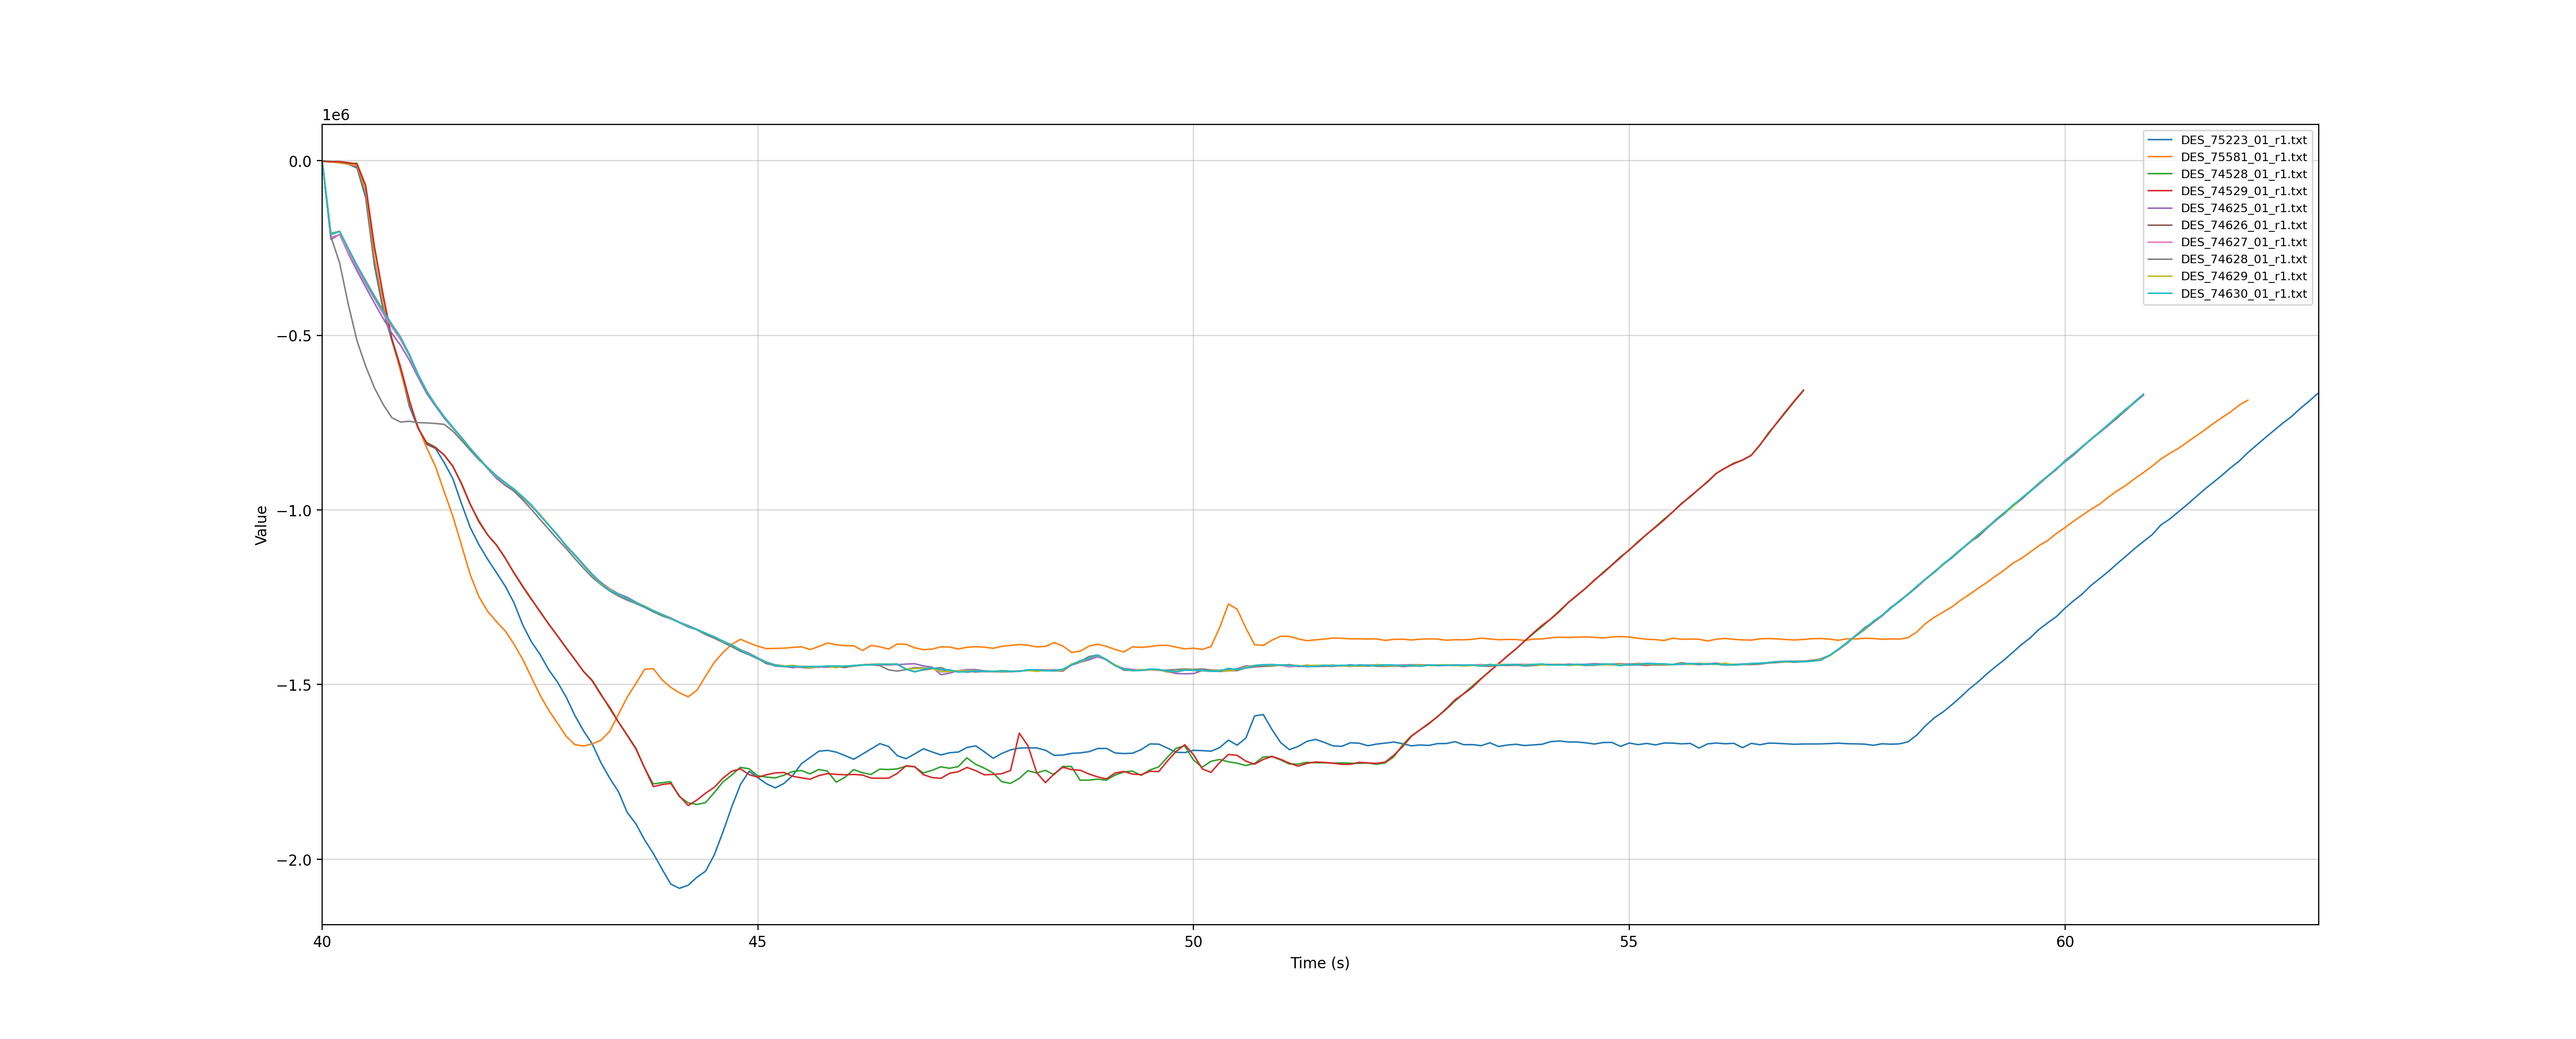
\includegraphics[width=\textwidth]{results/xgboost/75223_75581_vs_C23.png}
    \caption{Plasma current on discharges 75223 (blue) and 75581 (orange) compared to similar C23 non-disruptive discharges}
    \label{fig:ip_75223_75581}
\end{figure}

\subsubsection{Disruptive Discharges: 75273 and 75485}

Discharges 75273 and 75485 are disruptive discharges.\ \autoref{fig:ip_75273} and \autoref{fig:ip_75485} show the plasma current (in this case, in blue), compared with other similar C23 disruptive discharges. But as can be seen in \autoref{fig:ip_75273}, discharge 75273 is similar to some of non-disruptive discharges, so this is a good example of a discharge that can be misclassified as non-disruptive by some models.

\begin{figure}[H]
    \centering
    \includegraphics[width=\textwidth]{results/xgboost/75273_vs_C23.png}
    \caption{Plasma current on discharge 75273 (blue) compared to similar C23 disruptive discharges}
    \label{fig:ip_75273}
\end{figure}

\begin{figure}[H]
    \centering
    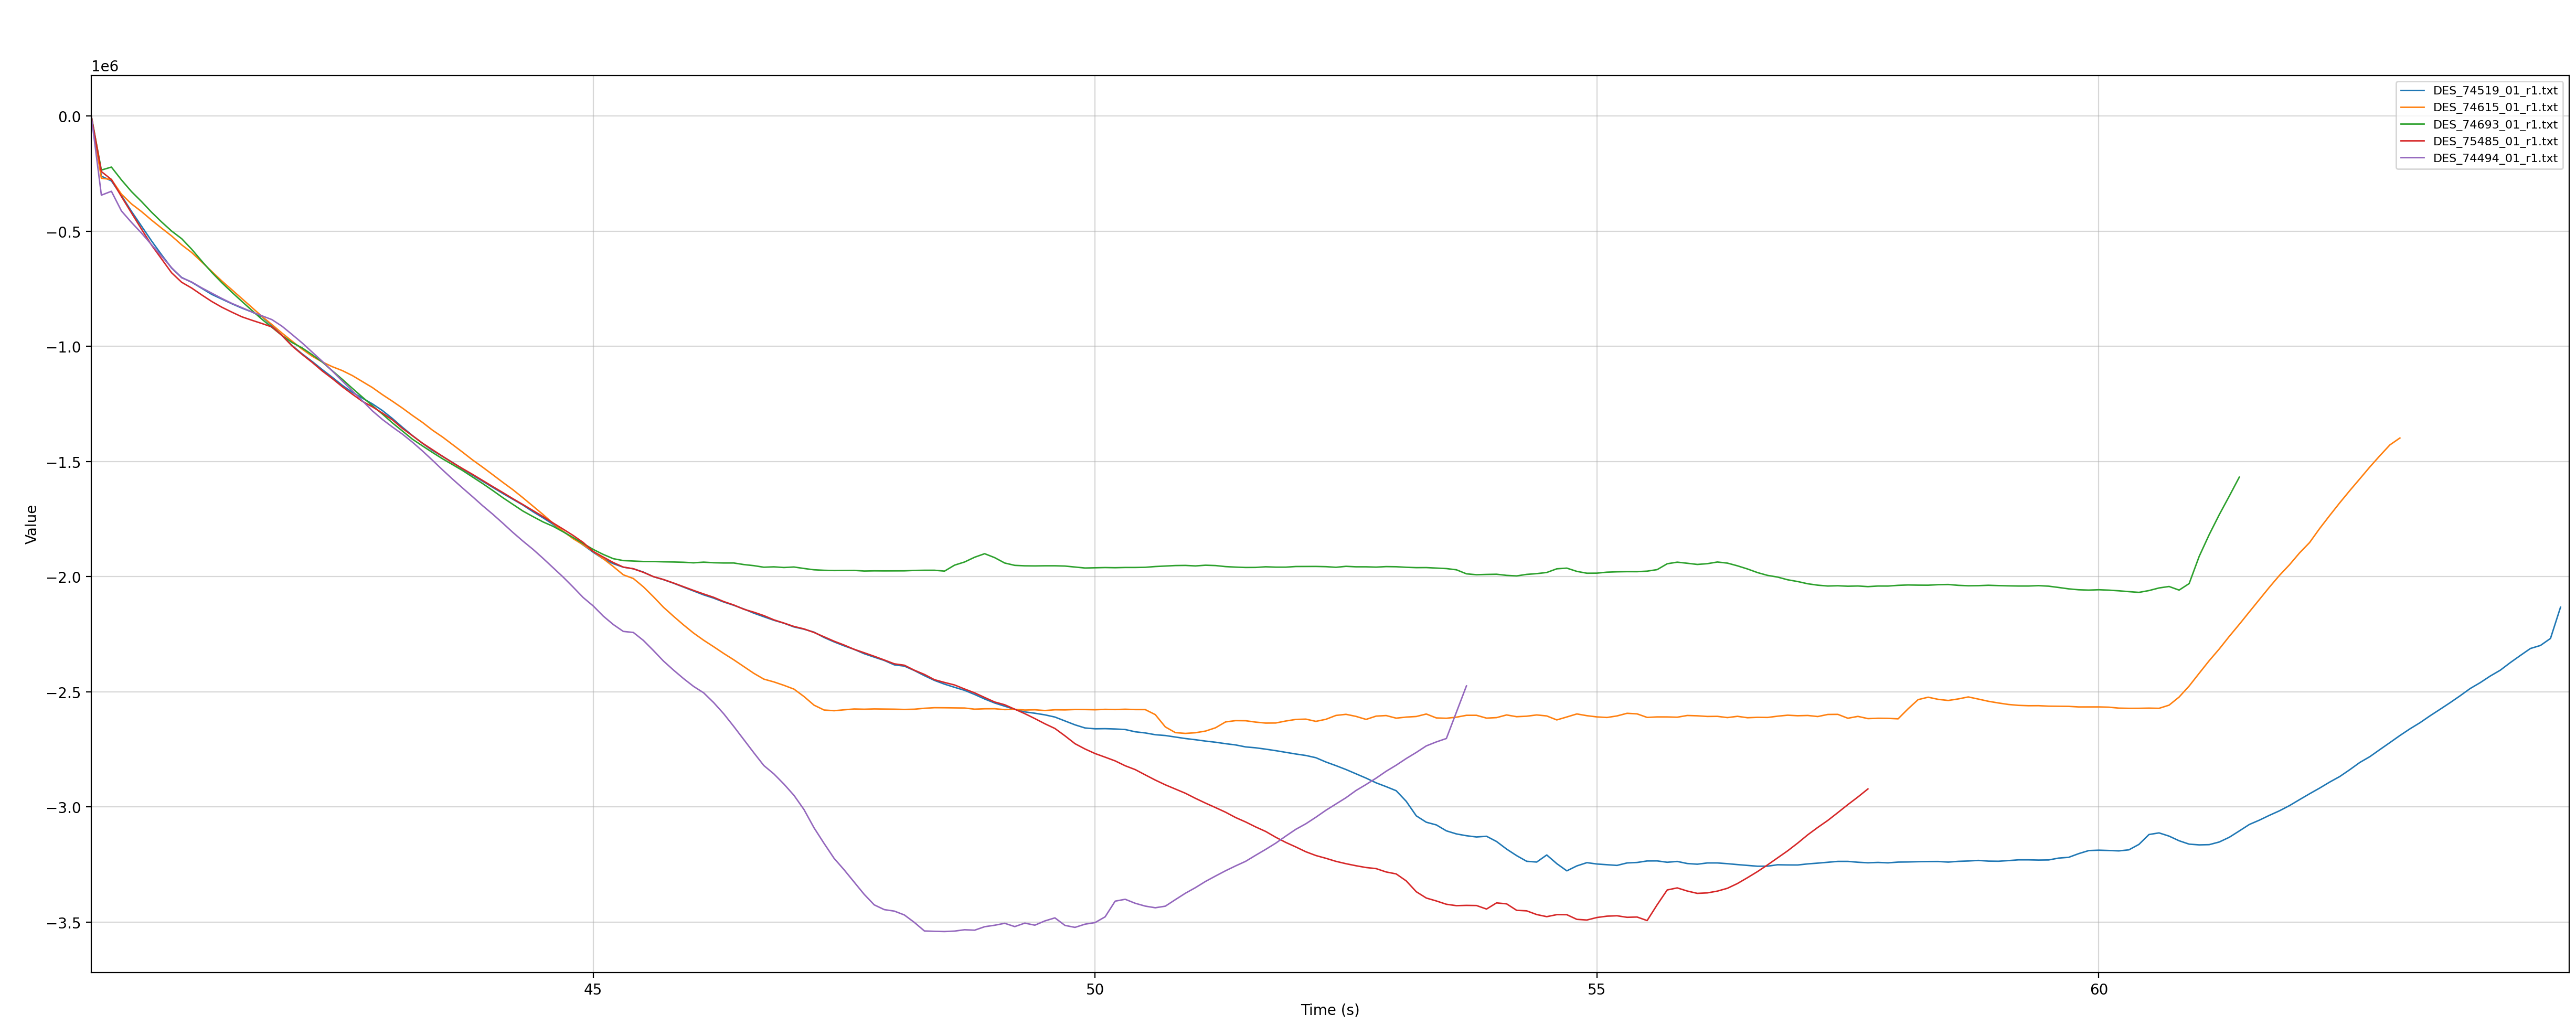
\includegraphics[width=\textwidth]{results/xgboost/75485_vs_C23.png}
    \caption{Plasma current on discharge 75485 (red) compared to similar C23 disruptive discharges}
    \label{fig:ip_75485}
\end{figure}

\begin{figure}[H]
    \centering
    \includegraphics[width=\textwidth]{results/iforest/75273_vs_C23.png}
    \caption{Plasma current on discharge 75273 (blue) compared to similar C23 non-disruptive discharges}
    \label{fig:iforest-75273-c23}
\end{figure}

\subsection{\acs{SVM}: \acs{APODIS} algorithm}

The \ac{APODIS} algorithm is a well known algorithm for anomaly detection in plasma discharges. It is important to note that this project does not aim to improve the \ac{APODIS} algorithm, but to implement it to compare its performance with other models.\ \autoref{fig:svm-config} shows the configuration for the \ac{SVM} model, which uses the default threshold of 0, and no \textit{count threshold}. As \autoref{sec:svm-implementation} describes, this model is not trained with the C23 campaign, but with a subset of the discharges, so these results are not directly comparable with the other models and shall be interpreted as a reference point.

\begin{figure}[H]
    \centering
    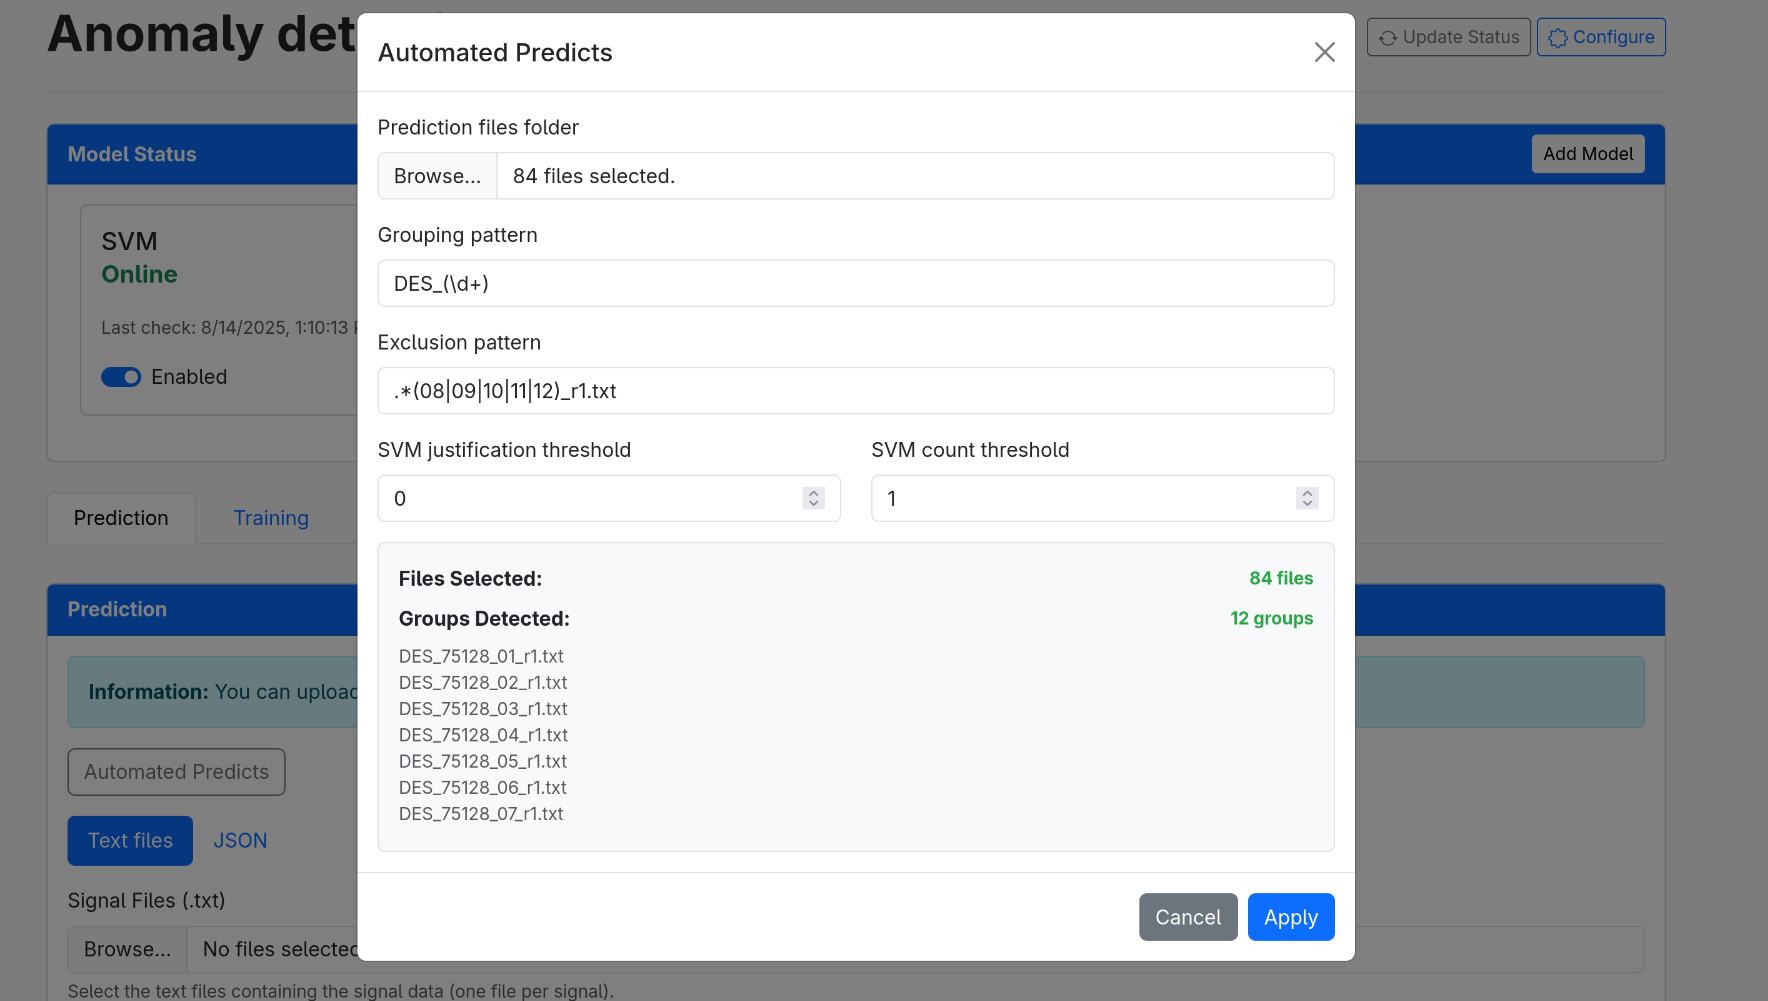
\includegraphics[width=\textwidth]{results/svm.png}
    \caption{SVM configuration}
    \label{fig:svm-config}
\end{figure}

\autoref{fig:svm-75223} and \autoref{fig:svm-75581} show the predictions of the \ac{SVM} model for discharges 75223 and 75581, respectively. In both cases, the model does not trigger any alert, as expected, since these are non-disruptive discharges. Even though, the distance to the separation hyperplane becomes narrow on window 300 for discharge 75223. 

\begin{figure}[H]
    \centering
    \includegraphics[width=\textwidth]{results/svm/75223.png}
    \caption{SVM prediction for discharge 75223 (non-disruptive)}
    \label{fig:svm-75223}
\end{figure}

\begin{figure}[H]
    \centering
    \includegraphics[width=\textwidth]{results/svm/75581.png}
    \caption{SVM prediction for discharge 75581 (non-disruptive)}
    \label{fig:svm-75581}
\end{figure}

\autoref{fig:svm-75273} and \autoref{fig:svm-75485} show the predictions of the \ac{SVM} model for disruptive discharges 75273 and 75485, respectively. In both cases, the model triggers alerts, correctly identifying the discharges as anomalous. The alerts are triggered around window 200 for discharge 75273, and around window 300 for discharge 75485. At discharge 75273, model correctly identifies the discharge as disruptive, but, due to the limited training data, discharge returns to a non-disruptive state.  

\begin{figure}[H]
    \centering
    \includegraphics[width=\textwidth]{results/svm/75273.png}
    \caption{SVM prediction for discharge 75273 (disruptive)}
    \label{fig:svm-75273}
\end{figure}

\begin{figure}[H]
    \centering
    \includegraphics[width=\textwidth]{results/svm/75485.png}
    \caption{SVM prediction for discharge 75485 (disruptive)}
    \label{fig:svm-75485}
\end{figure}

\subsection{XGBoost}

XGBoost implementation uses the features described in \autoref{subsubsec:xgboost}, which includes features from the current window and past windows as a tendency. This approach allows the model to have a better understanding of the discharge behavior over time, but also makes the model more rigid to changes in the discharge pattern. Additionally, model is trained with the C23 campaign and tested with the C24 campaign, which leads to a model that detects anomalies in the C24 campaign, but with some false positives because of the differences between the two campaigns, as explained in \autoref{apx:campaigns}. To reduce the false positives, orchestrator is configured to use a \textit{count threshold}, which means that more than one window must be labeled as anomalous in order to trigger an alert. 

Using the microservice approach, two XGBoost models are deployed, both with the same C23 training data, but while \texttt{xgboost\_2} uses a \textit{count threshold} of 2, \texttt{xgboost\_3} uses a \textit{count threshold} of 3. The automated predicts configuration is shown in \autoref{fig:xgboost-config}.

Increasing the \textit{count threshold} highly reduces the number of false positives, but also increases the lead time, as more windows must be labeled as anomalous before triggering an alert. With these settings, both models detect anomalies with any false negatives, but with some false positives, as explained in the next sections.

\begin{figure}[H]
    \centering
    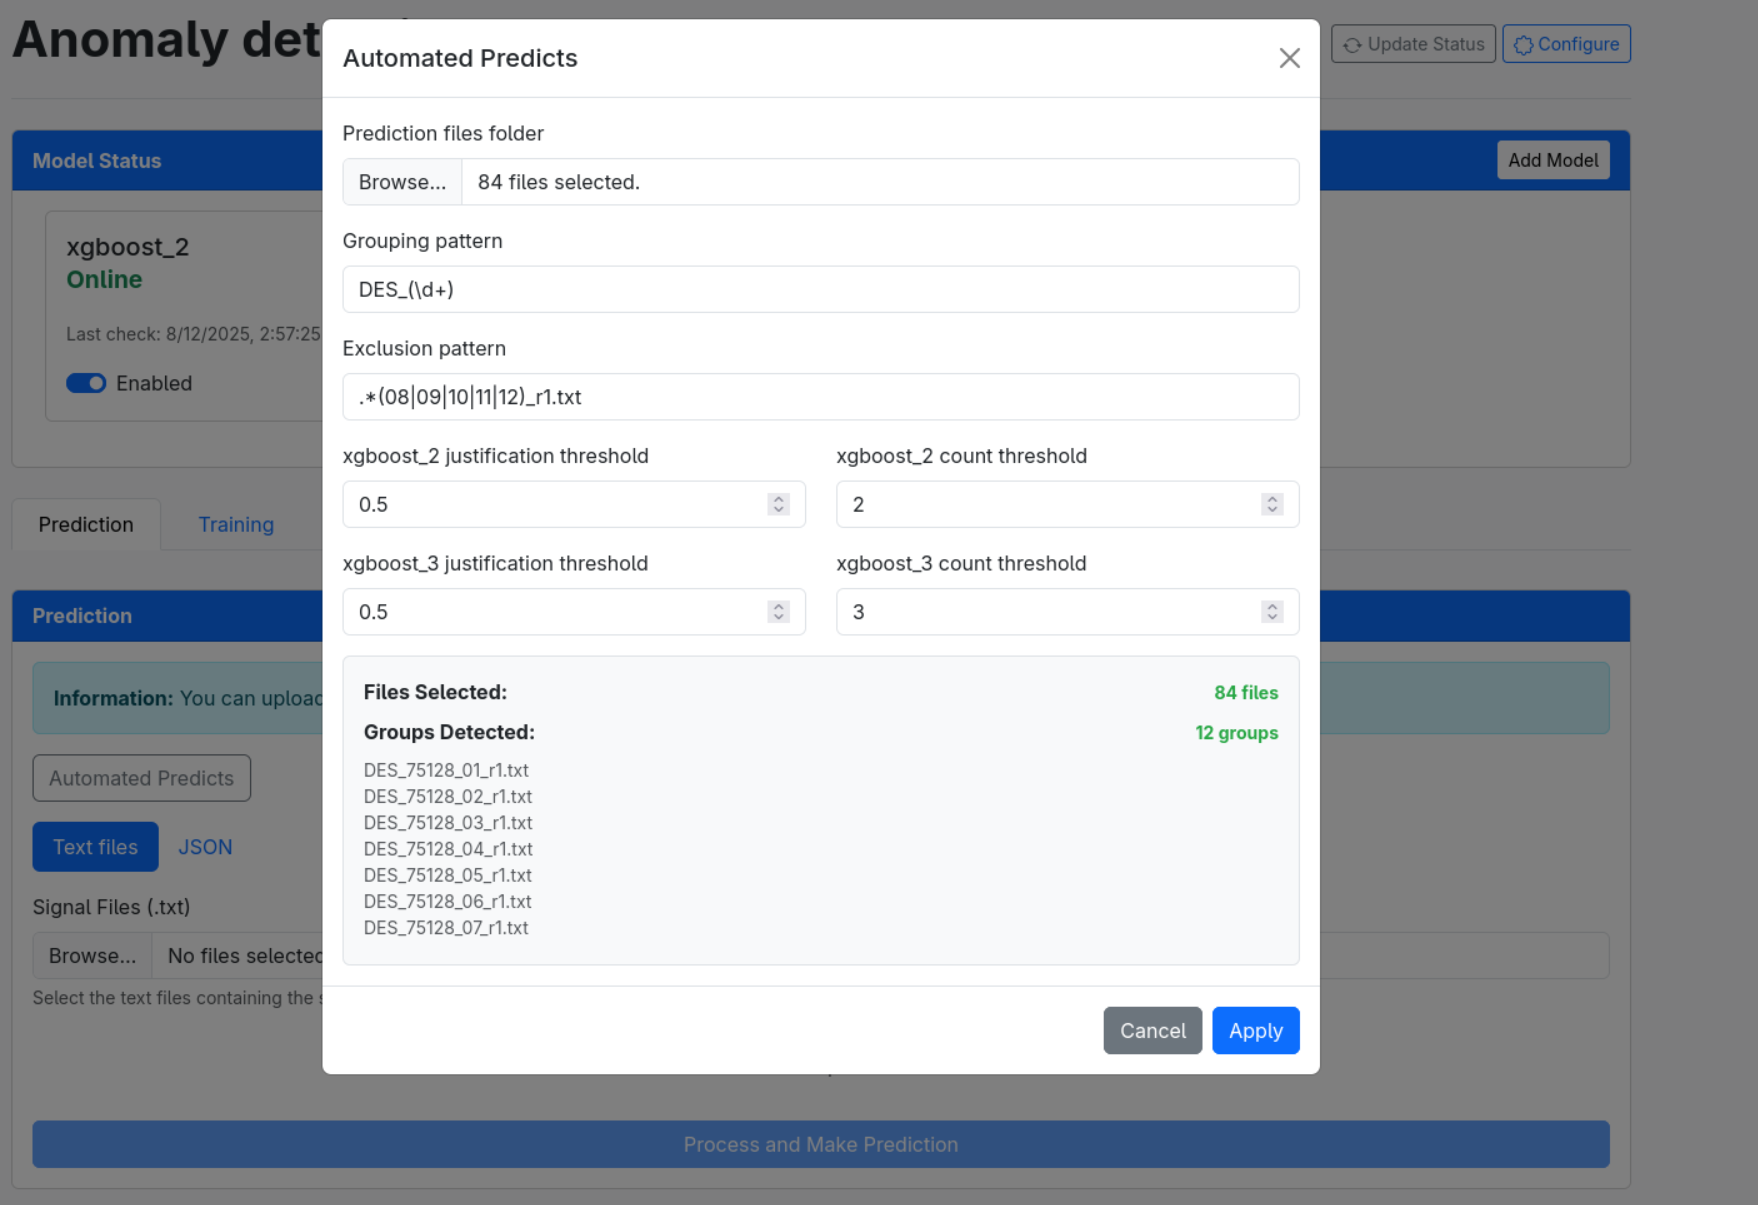
\includegraphics[width=\textwidth]{results/xgboost.png}
    \caption{XGBoost configuration}
    \label{fig:xgboost-config}
\end{figure}

\autoref{fig:xgboost-75223} shows both models predictions for discharge 75223, where the \texttt{xgboost\_2} alerts are represented in green, while the \texttt{xgboost\_3} alerts are in pink. There are also lines that reach the maximum value, and represent when the threshold has been reached. As can be seen, the \texttt{xgboost\_2} model triggers an alert around window 700, while the \texttt{xgboost\_3} model does not trigger any alert.\ \autoref{fig:xgboost-75581} shows the predictions for discharge 75581, where none of the models trigger an alert, as expected, since this is a non-disruptive discharge.

\begin{figure}[H]
    \centering
    \includegraphics[width=\textwidth]{results/xgboost/75223.png}
    \caption{XGBoost prediction for discharge 75223 (non-disruptive)}
    \label{fig:xgboost-75223}
\end{figure}

\begin{figure}[H]
    \centering
    \includegraphics[width=\textwidth]{results/xgboost/75581.png}
    \caption{XGBoost prediction for discharge 75581 (non-disruptive)}
    \label{fig:xgboost-75581}
\end{figure}

\autoref{fig:xgboost-75273} and \autoref{fig:xgboost-75485} show the predictions of both models for disruptive discharges. In this case, both models trigger many alerts (\texttt{xgboost\_3} alerts are on top of \texttt{xgboost\_2} alerts), correctly identifying the discharges as anomalous.

\begin{figure}[H]
    \centering
    \includegraphics[width=\textwidth]{results/xgboost/75273.png}
    \caption{XGBoost prediction for discharge 75273 (disruptive)}
    \label{fig:xgboost-75273}
\end{figure}

\begin{figure}[H]
    \centering
    \includegraphics[width=\textwidth]{results/xgboost/75485.png}
    \caption{XGBoost prediction for discharge 75485 (disruptive)}
    \label{fig:xgboost-75485}
\end{figure}

\subsubsection{False positives: 75128}

Discharge 75128 is a non-disruptive discharge, but \texttt{xgboost\_2} and \texttt{xgboost\_3} models trigger alerts, labeling this discharge as anomalous. This is caused because of the high correlation between this discharge and some of the disruptive discharges used for training the model, as shown in \autoref{fig:ip_75128}, where the plasma current of discharge 75128 (in blue) is compared with similar C23 disruptive discharges. Even though the discharge is also similar to some of non-disruptive discharges, weigh of the disruptive discharges is higher, as shown in \autoref{eq:gbdt-objective}, where $w_i$ is $\approx$ 11 times higher for disruptive discharges than for non-disruptive discharges, as this is the ratio of the number of disruptive windows to the number of non-disruptive windows in the training set. This leads to a model that is more sensitive to disruptive discharges, but also more prone to false positives when the discharge is similar to a disruptive discharge. 

\autoref{fig:xgboost-75128} shows the predictions of both models for discharge 75128.

\begin{figure}[H]
    \centering
    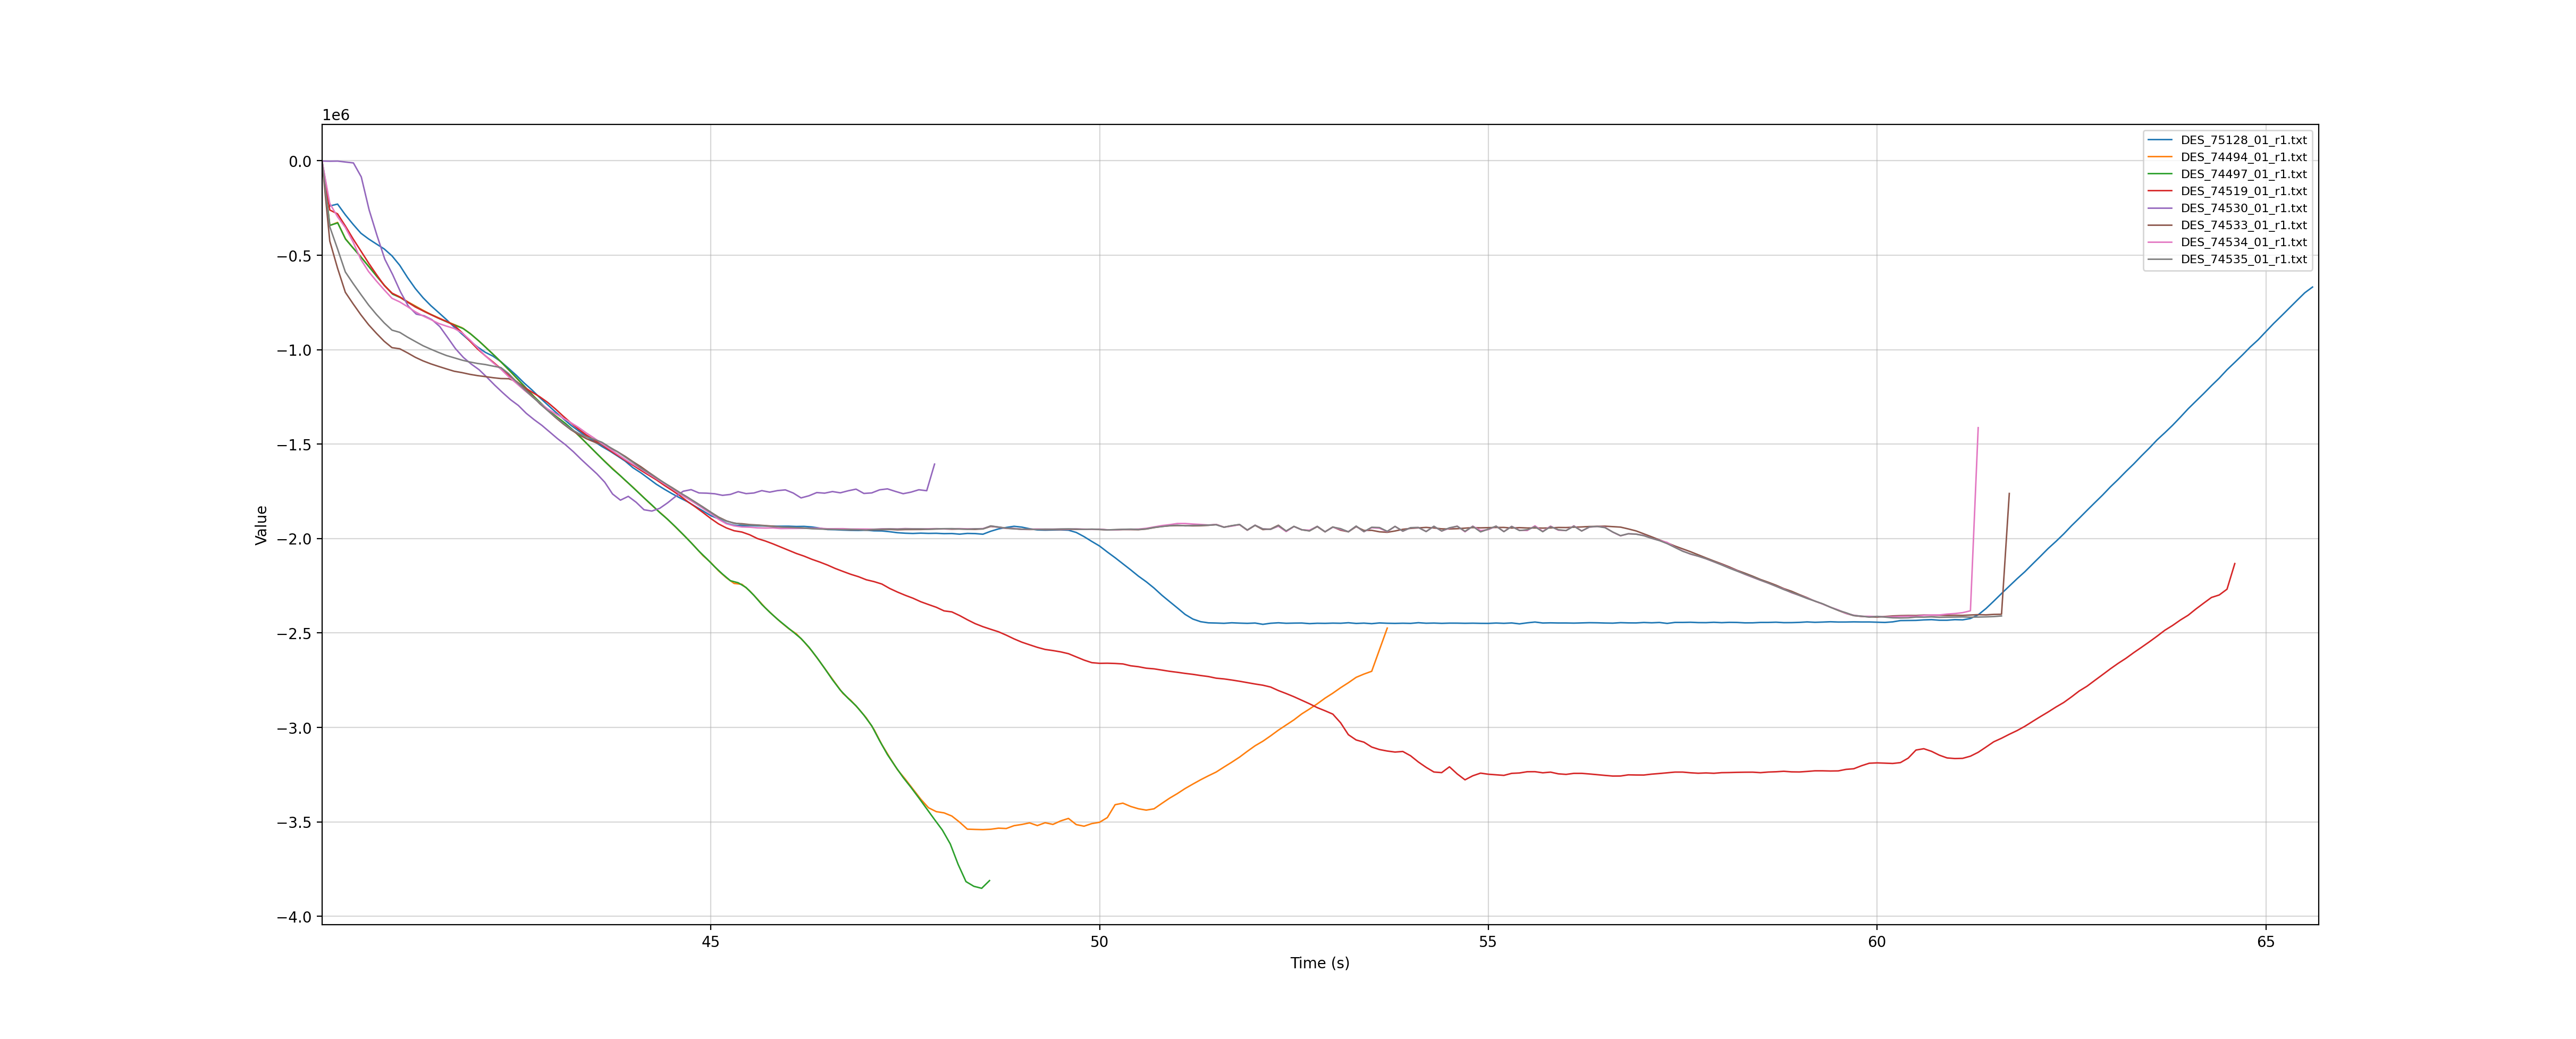
\includegraphics[width=\textwidth]{results/xgboost/75128_vs_C23.png}
    \caption{Plasma current on discharge 75128 (blue) compared to similar C23 disruptive discharges}
    \label{fig:ip_75128}
\end{figure}

\begin{figure}[H]
    \centering
    \includegraphics[width=\textwidth]{results/xgboost/75128.png}
    \caption{XGBoost prediction for discharge 75128}
    \label{fig:xgboost-75128}
\end{figure}

\subsection{IForest}

This section presents the results of the Isolation Forest model, which is explained in \autoref{sec:iforest-implementation}. This model is configured with the parameters shown in \autoref{fig:iforest-config}, where the \textit{justification threshold} is set to 0, and a \textit{count threshold} of 2 is used. 

\begin{figure}[H]
    \centering
    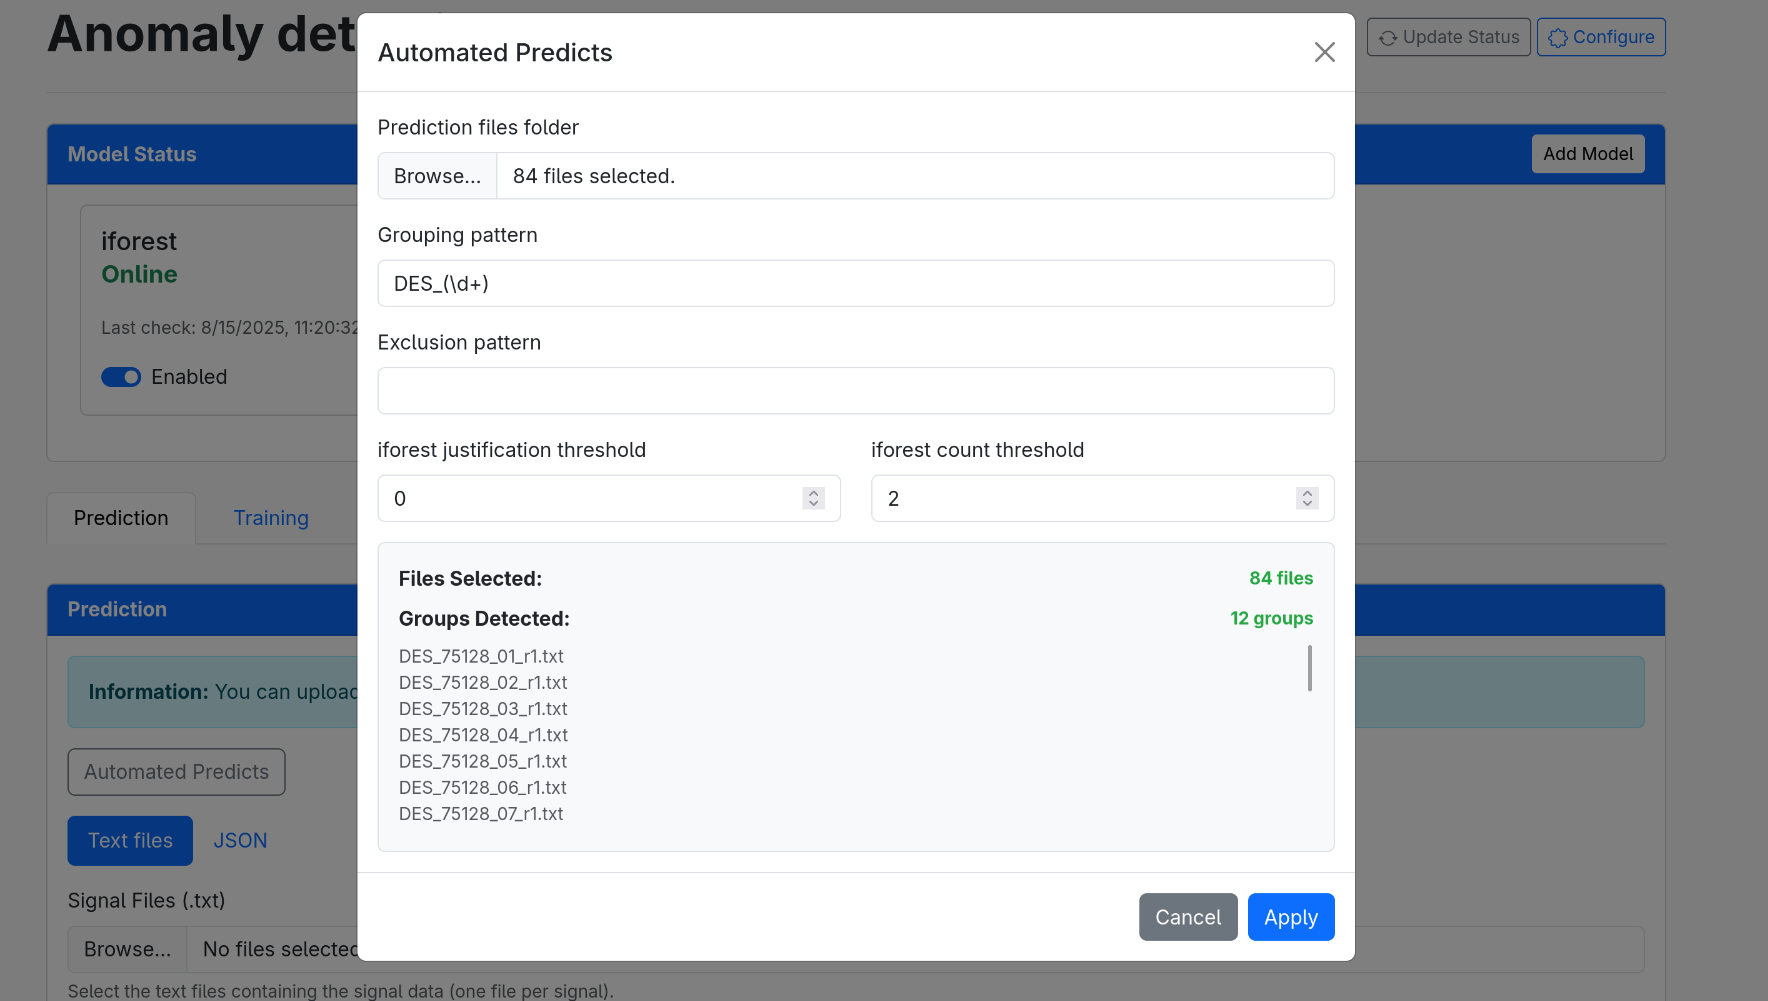
\includegraphics[width=\textwidth]{results/iforest.png}
    \caption{Isolation Forest configuration}
    \label{fig:iforest-config}
\end{figure}


The model is trained with the non-disruptive discharges from the C23 campaign, and outperforms the previous xgboost model in accuracy metrics, as it does not trigger false positives on non-disruptive discharges, but it has a lower lead time, as it triggers alerts later than the xgboost model.

\autoref{fig:iforest-75223} and \autoref{fig:iforest-75581} show the predictions of the Isolation Forest model for non-disruptive discharges 75223 and 75581, respectively. In both cases, the model does not trigger any alert, correctly identifying these discharges as non-disruptive. On discharge 75223, the justification threshold is reached at the beginning of the discharge, but the model does not trigger an alert, as the \textit{count threshold} is not reached. This behavior highlights the importance of the \textit{count threshold} in reducing false positives, as the model is more conservative in its predictions.

\begin{figure}[H]
    \centering
    \includegraphics[width=\textwidth]{results/iforest/75223.png}
    \caption{\ac{IForest} prediction for discharges 75223 (non-disruptive)}
    \label{fig:iforest-75223}
\end{figure}

\begin{figure}[H]
    \centering
    \includegraphics[width=\textwidth]{results/iforest/75581.png}
    \caption{\ac{IForest} prediction for discharges 75581 (non-disruptive)}
    \label{fig:iforest-75581}
\end{figure}

\autoref{fig:iforest-75273}  shows the predictions of the Isolation Forest model for disruptive discharge 75273. In this case, model is not fast enough to trigger an alert. It can be seen that the model starts to increase the threshold value, and last window is labeled as anomalous, but the alert is not triggered until the end of the discharge. This behavior is caused because the model is trained with non-disruptive discharges, and as \autoref{fig:iforest-75273-c23} shows, this discharge shows a non-disruptive pattern until the end of the discharge. Discharge 75485 is correctly identified as disruptive, as shown in \autoref{fig:iforest-75485}.

\begin{figure}[H]
    \centering
    \includegraphics[width=\textwidth]{results/iforest/75273.png}
    \caption{\ac{IForest} prediction for discharges 75273 (disruptive)}
    \label{fig:iforest-75273}
\end{figure}

\begin{figure}[H]
    \centering
    \includegraphics[width=\textwidth]{results/iforest/75485.png}
    \caption{\ac{IForest} prediction for discharges 75485 (disruptive)}
    \label{fig:iforest-75485}
\end{figure}

\subsection{XGBoost vs Isolation Forest}

XGboost and Isolation Forest are decision tree based models, but they have different approaches to anomaly detection. XGBoost uses a gradient boosting approach, where the model is trained with a set of features and tries to minimize the error in the predictions. On the other hand, Isolation Forest is an unsupervised model that tries to isolate anomalies by randomly selecting features and splitting the data.

It has been already shown that XGBoost triggers a false positive on discharge 75128, while \autoref{fig:iforest-75128} demonstrates that Isolation Forest does not trigger any alert on this discharge, correctly identifying it as non-disruptive. This is because the Isolation Forest model is trained with non-disruptive discharges, and it is more conservative in its predictions, while XGBoost is more sensitive to disruptive discharges, leading to false positives. 

\begin{figure}[H]
    \centering
    \includegraphics[width=\textwidth]{results/iforest/75128.png}
    \caption{\ac{IForest} prediction for discharge 75128}
    \label{fig:iforest-75128}
\end{figure}

This behavior is clearly shown in \autoref{fig:iforest-vs-xgboost-75543}, which is a disruptive discharge, but whereas XGBoost triggers many alerts on the central part of the discharge, Isolation Forest is more conservative, and only triggers an alert at the end of the discharge.

\begin{figure}[H]
    \centering
    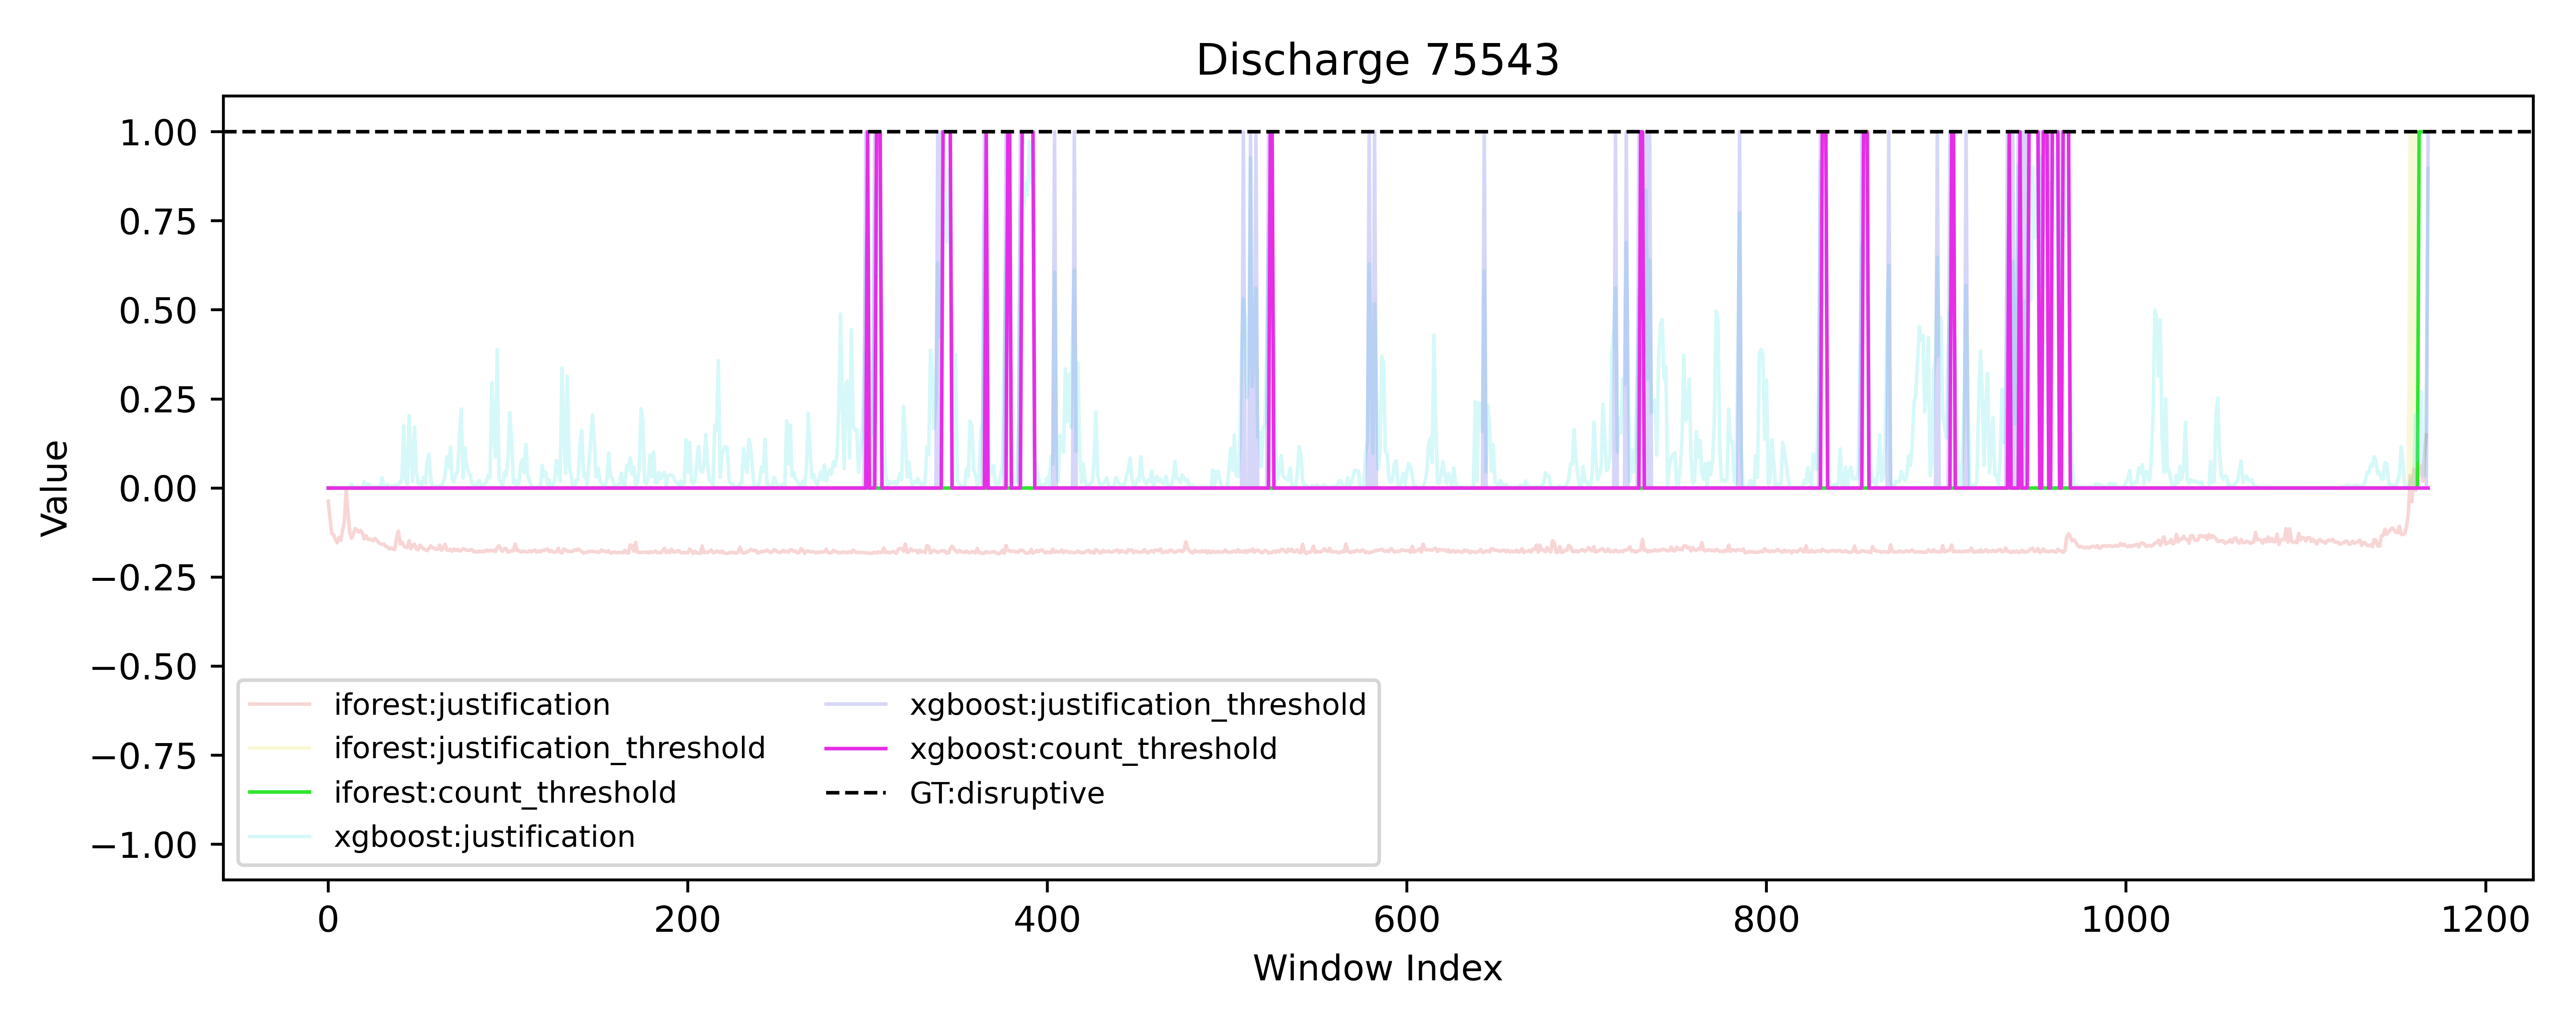
\includegraphics[width=\textwidth]{results/iforest_vs_xgboost/75543.png}
    \caption{Comparison of XGBoost and Isolation Forest predictions for discharge 75543}
    \label{fig:iforest-vs-xgboost-75543}
\end{figure}

\subsubsection{CNN-FFT}

\begin{figure}[H]
    \centering
    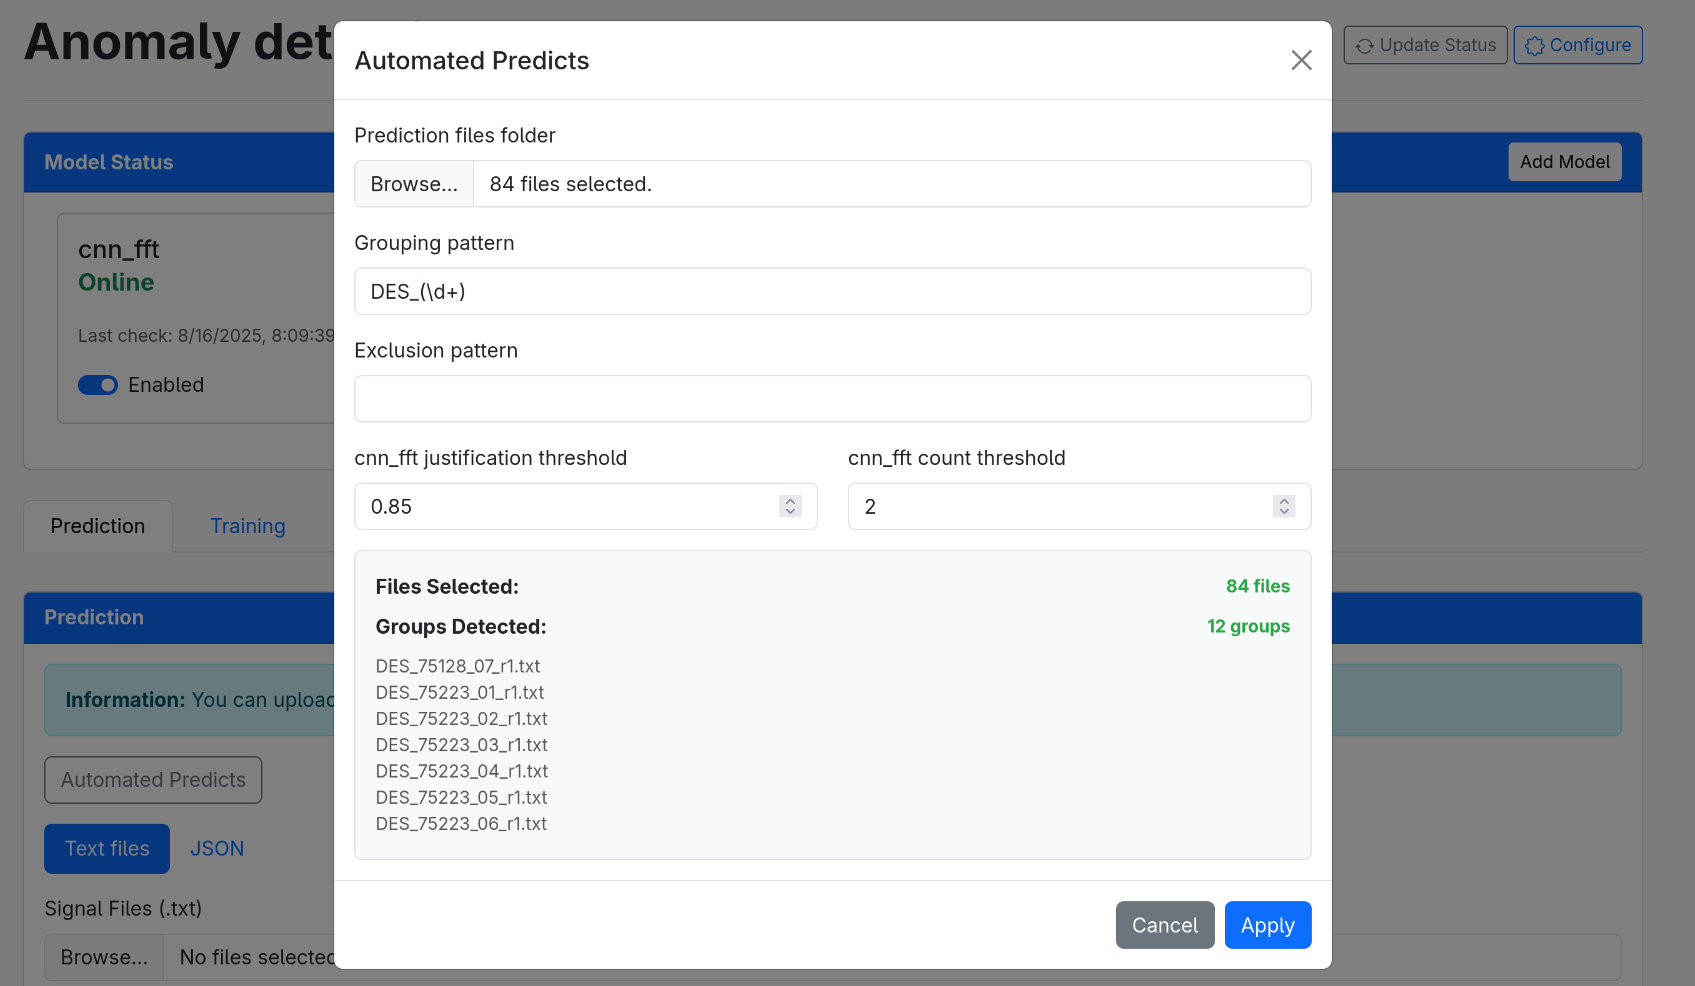
\includegraphics[width=\textwidth]{results/cnn_fft.png}
    \caption{CNN-FFT configuration}
    \label{fig:cnn-fft-config}
\end{figure}


\begin{figure}[H]
    \centering
    \includegraphics[width=\textwidth]{results/cnn_fft/75223.png}
    \caption{CNN-FFT prediction for discharge 75223 (non-disruptive)}
    \label{fig:cnn-fft-75223}
\end{figure}

\begin{figure}[H]
    \centering
    \includegraphics[width=\textwidth]{results/cnn_fft/75581.png}
    \caption{CNN-FFT prediction for discharge 75581 (non-disruptive)}
    \label{fig:cnn-fft-75581}
\end{figure}

\begin{figure}[H]
    \centering
    \includegraphics[width=\textwidth]{results/cnn_fft/75273.png}
    \caption{CNN-FFT prediction for discharge 75273 (disruptive)}
    \label{fig:cnn-fft-75273}
\end{figure}

\begin{figure}[H]
    \centering
    \includegraphics[width=\textwidth]{results/cnn_fft/75485.png}
    \caption{CNN-FFT prediction for discharge 75485 (disruptive)}
    \label{fig:cnn-fft-75485}
\end{figure}

